\documentclass[11pt]{report}
\usepackage{graphicx}
\usepackage{amssymb}
\usepackage{amsthm}
\usepackage{amsmath}
\usepackage{fullpage}
\usepackage{tikz}
\usetikzlibrary{positioning}
\tikzset{node distance=5cm, auto}
\usepackage{cite}
\DeclareGraphicsRule{.tif}{png}{.png}{`convert #1 `dirname #1`/`basename #1 .tif`.png}

\newtheorem{thm}{Theorem}
\newtheorem{prop}{Proposition}
\newtheorem{lemma}{Lemma}
\newtheorem{definition}{Definition}
\newtheorem{proposition}{Proposition}

%%%%%%%%%%%%%%%%%%%%%%%%%%%%%%%%%%%%
%%%%%%%%%%%%%%%%%%%%%%%%%%%%%%%%%%%%
\newcommand{\Q}{\mathbb{Q}}
\newcommand{\Z}{\mathbb{Z}}
\newcommand{\C}{\mathbb{C}}
\newcommand{\R}{\mathbb{R}}
\newcommand{\N}{\mathbb{N}}
\newcommand{\M}{\mathcal{M}}
\newcommand{\Zp}{\mathbb{Z}/p\mathbb{Z}}
\newcommand{\ZP}{\mathbb{Z}/P\mathbb{Z}}
\newcommand{\Zn}{\mathbb{Z}/n\mathbb{Z}}
\newcommand{\Zm}{\mathbb{Z}/m\mathbb{Z}}
\newcommand{\bl}{\ & \ & \\}
\newcommand{\eql}{\ & = &}
\newcommand{\ba}{\\ \begin{array}{rcl}}
\newcommand{\ea}{\end{array} \\}
\newcommand{\claim}{\underline{Claim}: \ }
\newcommand{\pf}{\underline{Proof of Claim}: \\ }
\newcommand{\mat}{\left[\begin{array}{cc} a & b \\ c & d \end{array}\right]}
\newcommand{\lra}{\longrightarrow}
\newcommand{\mf}{\mathfrak}
\newcommand{\inv}{^{-1}}
\newcommand{\ML}{\mathcal{L}}
\newcommand{\LM}{\mathcal{L}}
\newcommand{\LMEF}{\mathcal{L}(E;F)}
\newcommand{\Mnn}{M(n\times n)}
\newcommand{\OnR}{O(n;\R)}
\newcommand{\XM}{\mathfrak{X}(M)}
\newcommand{\eps}{\epsilon}
\newcommand{\CM}{C^{\infty}(M)}
\newcommand{\ddt}{\frac{d}{dt}}
\newcommand{\dds}{\frac{d}{ds}}
\newcommand{\Zhat}{\hat{\mathbb{Z}}}
\newcommand{\coker}{\text{coker}}
\newcommand{\Hom}{\text{Hom}}
\newcommand{\End}{\text{End}}
\newcommand{\Aut}{\text{Aut}}
\newcommand{\Tr}{\text{Tr}}
\newcommand{\ra}{\rightarrow}
\newcommand{\Ra}{\Rightarrow}
\newcommand{\mfp}{\mathfrak{p}}
\newcommand{\mfq}{\mathfrak{q}}
\newcommand{\mfm}{\mathfrak{m}}
\newcommand{\Ap}{A_{\mathfrak{p}}}
\newcommand{\OK}{\mathcal{O}_k}
\newcommand{\Zx}{\mathbb{Z}[x]}
\newcommand{\Zy}{\mathbb{Z}[y]}
\newcommand{\Zxn}{\mathbb{Z}[x_1,\ldots,x_n]}
\newcommand{\Zxy}{\mathbb{Z}[x,y]}
\newcommand{\Zpxy}{\mathbb{Z}/p\mathbb{Z}[x,y]}
\newcommand{\beq}{\begin{equation*}}
\newcommand{\eeq}{\end{equation}}
\newcommand{\GB}{Gr\"obner basis }
\newcommand{\bigO}{\mathcal{O}}
%\setlength{\parindent}{0cm}        % \noindent everywhere!
%%%%%%%%%%%%%%%%%%%%%%%%%%%%%%%%%%%%
%%%%%%%%%%%%%%%%%%%%%%%%%%%%%%%%%%%%

\setcounter{tocdepth}{2} %show up to subsections in table of contents
\setcounter{chapter}{-1} %first chapter should be 0

\title{Approaches to Homomorphic Encryption Using Polynomial Rings and the Chinese Remainder Theorem}
\author{Benjamin T. LeVeque}
\date{\today}         

\begin{document}
\maketitle


\tableofcontents

\newpage

%%%%%%%%%%%%%%%%%%%%%%%%
%%%%%%%%%%%%%%%%%%%%%%%%
\chapter{Acknowledgements}


%%%%%%%%%%%%%%%%%%%%%%%%
%%%%%%%%%%%%%%%%%%%%%%%%
\chapter{Introduction and background}

\section{Introduction}

In an age of ubiquitous computing, digital security is an important aspect of everyday life. Cryptography is already a pervasive concept, providing privacy for everything from email communication to financial transactions. As computations involving large data sets become more expensive and time-consuming, and as the need for data storage increases, cloud computing has rapidly become a platform to which people and institutions alike turn for their computational needs. With this rise in popularity comes the need for a new class of security protocols that allow data to be stored in encrypted form yet manipulated in a meaningful way by third parties. In this thesis, we consider two such cryptographic schemes. We discuss the motivation behind them, analyze their security, and present data regarding both their security and efficiency. We also provide implementations of the systems in question in C++ and explain the code's design.

Two goals in the very close periphery throughout the development of this project have been reproducibility and accessibility. In this vein, the implementations produced and the data generated are posted in a public repository on Github at https://github.com/bleveque/HomEnc, and a website accompanying the project can be found at (INSERT ADDRESS).

\section{Introduction to cryptographic concepts and terminology} 

Before explaining and analyzing specific schemes, we give a brief background on some common cryptographic concepts. A \emph{cryptosystem} is a collection of procedures that allow a user to securely map a \emph{message} (also called a \emph{plaintext}) $m$ to a \emph{cipertext} $c$ such that the reverse map can only be easily computed given some private information, called a \emph{secret key}. The map taking a message to a ciphertext is referred to as an \emph{encryption function} and will be denoted by $e$, while the reverse map is referred to as a \emph{decryption function} and will be denoted by $d$. The process of determining the secret key is known as \emph{key generation}, and the key generation function will be denoted by $KG$. The messages lie in some space, referred to as the \emph{message space} ($\M$), and the ciphertexts lie in a (possibly) different space, referred to as the \emph{ciphertext space} ($\mathcal{C}$), so we have
\begin{align*}
e: \M \lra \mathcal{C} \\
d: \mathcal{C} \lra \M \\
(d\circ e) = id_{\M}
\end{align*}
A cryptosystem is then given by a collection \[\{\M, \mathcal{C},  KG, e, d\}\] This information together tells us exactly where our messages are coming from and how to encrypt and decrypt them.

\label{Example1}To illustrate the construction above with a brief example, consider the cryptosystem defined by the following elements:
\begin{align*}
&\M = \Z \\
&\mathcal{C} = \Z \\
&KG \text{ gives a random integer } k>1 \\
&e: m \mapsto km \\
&d: c \mapsto c/k
\end{align*}
\noindent This simple scheme encrypts an integer message $m$ by taking its product with the secret key $k$. The resulting ciphertext can be decrypted by dividing by $k$: \[d(e(m)) = d(km) = m\] It is therefore well-defined to encrypt and decrypt a message. This scheme is not very secure, since the value of $k$ can be easily discovered by examining several message/ciphertext pairs, but it is illustrative of the basic ideas.

A lingering question might be ``my message is a regular sentence! how can the message space $\Z$ be of any use to me?'' The answer comes in the form of an invertible \emph{encoding function}. An encoding function is not meant to provide any extra security to our scheme; its sole purpose is to transform real messages into a format we can use in our encryption function. For example, we could encode a word by sending each letter to a number:
\begin{align*}
&a\mapsto 1 \\
&b\mapsto 2 \\
& \vdots \\
&z\mapsto 26
\end{align*}
so the word ``crypto'' would be encoded as the sequence of numbers 3-18-25-16-20-15. We could then use our encryption function on each of these numbers. When we decrypt the result, we will get the sequence of numbers back, and then we must perform the inverse of the encoding function to recover our word as a sequence of letters c-r-y-p-t-o.

\

\section{Introduction to homomorphic encryption}
\label{sec:intro_to_hom_enc}

The idea of a homomorphic cryptosystem extends the ideas presented above by adding an additional requirement to our definitions. To motivate this requirement, imagine you have a large collection of data points and want to compute their mean or standard deviation. You have have two options: you can either do this computation yourself at a potentially high computational cost, or you can delegate this work to another party and risk losing privacy by exposing your data.  The goal of fully homomorphic encryption is to minimize both potential costs by allowing secure delegation. In practice, this might mean being able to store data on the Cloud in an encrypted form such that a third party could still manipulate the data in a meaningful way. By meaningful, we simply mean that after they operate on our data, we can decrypt the result and obtain exactly the value their operations would have achieved on our original plaintext data. The following diagram illustrates this process:

\

\begin{center}
$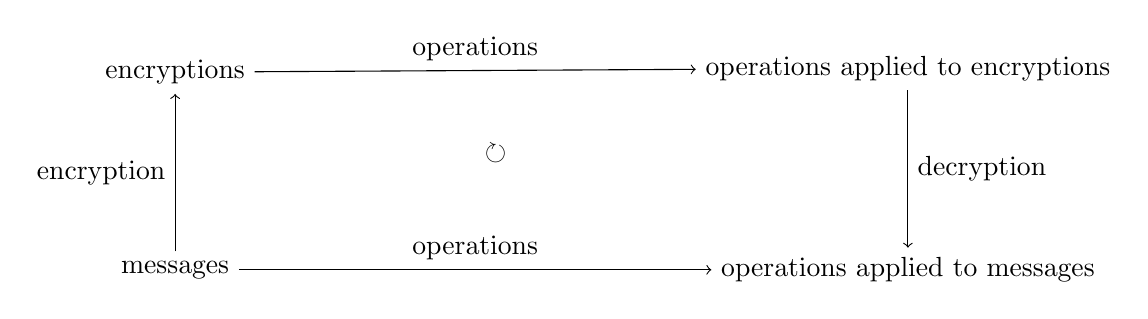
\begin{tikzpicture} \label{hom_diagram}
\node (m) {messages};
\node (fm) [right=6cm of m] {operations applied to messages};
\node (em) [above=2cm of m] {encryptions};
\node (fem) [above=2cm of fm] {operations applied to encryptions};
\node(circarr) [above right=1cm and 3cm of m]{$\circlearrowright$};
\draw[->] (m) to node {operations} (fm);
\draw[->] (fem) to node {decryption} (fm);
\draw[->] (m) to node {encryption} (em);
\draw[->] (em) to node {operations} (fem);
\end{tikzpicture}$
\end{center}

\

Homomorphic encryption ensures that we achieve the same result by traversing this diagram in either direction starting from our messages (i.e. the diagram is \emph{commutative}). More technically, by ``meaningful'' we mean that any combination of sums and products of encryptions decrypt to the corresponding sums and products of the original, unencrypted data (we call such a combination an \emph{arithmetic circuit}, or just a \emph{circuit}). If this condition holds, data could be encrypted, operated upon, and decrypted in a completely well-defined manner. What we are looking for, then, is an encryption function that is a \emph{ring homomorphism} from the message space $\M$ to the ciphertext space $\mathcal{C}$. Recall that a ring homomorphism is a map $\sigma: \M \rightarrow \mathcal{C}$ such that for any $x,y\in \M$, \[\sigma(x)+\sigma(y) = \sigma(x+y)\] \[\sigma(x) \sigma(y) = \sigma(xy)\] If our encryption function $e$, then, is a ring homomorphism, we could add or multiply two encryptions and the result would be the encryption of the sum or product of the corresponding plaintexts. A cryptosystem employing such an encryption function is said to give \emph{fully homomorphic encryption} (FHE). If the encryption function in question is homomorphic on most inputs, but is not guaranteed to give well-defined decryption after the application of every circuit, the scheme is said to provide \emph{somewhat homomorphic encryption}. Such a scheme might arise if the decryption function requires its input to be of a certain size, which the application of large circuits might exceed. For motivation, consider the following toy example.

\subsection{Example}
\label{Example2}First, we will construct a somewhat homomorphic encryption scheme, and then we will attempt to extend it to be fully homomorphic. Consider the message space $\M = \Z_{\geq 0}$ and choose as a secret key some prime number $p$. We will encrypt a message $m\in \M$ by setting $e(m) = m+ap$ for some random integer $a$. Decryption is then performed by reducing modulo $p$. As long as the message $m$ is less than $p$, this scheme is perfectly well defined, since
\begin{align*}
d(e(m)) &= m+ap \pmod{p}\\
              &= m
\end{align*}
The scheme is additively homomorphic for messages $m_1$ and $m_2$ if $m_1+m_2<p$ because we have
\begin{align*}
d(e(m_1)+e(m_2)) &= m_1+m_2+(a_1+a_2)p \pmod{p}\\
&= m_1+m_2
\end{align*}
and multiplicatively homomorphic if $m_1m_2<p$, since
\begin{align*}
d(e(m_1)e(m_2)) &= m_1m_2+(m_1a_2+m_2a_1+a_1a_2p)p \pmod{p}\\
&= m_1m_2
\end{align*}
However, if any of the messages above satisfy $m\geq p$, then $d(e(m))$ will no longer equal $m$, but will be the reduction of $m$ modulo $p$. We can attempt to avoid this problem by encrypting only messages less than $p$, but once we start considering circuits applied to encryptions, this idea shows its flaws. For example, we might want the sum of two encryptions of $p-1$ to decrypt to $2p-2$, but it would decrypt instead to
\[2p-2 \pmod{p} = p-2 \]
Another solution is to recognize the limitations of the system and include as a part of the system's protocol a bound on the number of additions and multiplications that can be performed on encryptions before the result should be decrypted. 

To make this scheme fully homomorphic, we could set $\M = \Zp$, since in this case, reducing modulo $p$ during decryption is consistent with the structure of the message space. However, it is perhaps unnatural for messages to live in $\Zp$, since when we compute circuits such as the computation of standard deviations, we don't want to reduce modulo $p$ at any point during the computation. In this case, it may be best to accept the limitations of the somewhat homomorphic scheme above and work within its framework.

It should be mentioned, as well, that the scheme above is just a ``toy'' example because as in the case of the example on page \pageref{Example1}, it is very insecure. Suppose an eavesdropper asked us to encrypt the message $m=0$ using this system. The result would be a multiple of $p$. If we were asked to perform many such encryptions, the eavesdropper would end up with a collection of multiples of $p$. With this information, he could very quickly compute the greatest common divisor of these values using the Euclidean Algorithm, and the result would likely be $p$ itself. Using $p$, the eavesdropper could then decrypt any message he pleased by simply reducing it modulo $p$. This type of attack---using encryptions of the message $0$ to reveal an essential feature of the structure of the scheme itself---will appear again, and is a necessary threat to consider when formulating encryption schemes. This attack and others are discussed in the appendix.

%%%%%%%%%%%%%%%%%%%%%%%%%%%
%%%%%%%%%%%%%%%%%%%%%%%%%%%
\chapter{Schemes under investigation}

\section{Introduction to present work}

\
In his 2009 dissertation~\cite{gentry-thesis}, Craig Gentry presented the first secure fully homomorphic encryption scheme. His construction was based on the theory of ideal lattices (ideals in quotient polynomial rings), and it represented a major breakthrough as a proof-of-concept and started a rapid-pace movement towards creating an \emph{efficient} fully homomorphic scheme. This thesis will present two cryptosystems that show promise as either somewhat or fully homomorphic encryption schemes and explore their security and efficiency.

The first, which is formulated entirely over the integers (and quotient rings thereof), relies on the hardness of making $N$ consecutive correct choices, where each choice is between two values. We will refer to this as ``choice-based encryption'' (CBE). The second, which is formulated over multivariate polynomial rings, relies on the hardness of the ideal membership problem (IMP) in this setting. Similar schemes in the past---sometimes referred to as \emph{Polly Cracker} schemes after their introduction by Koblitz and Fellows in~\cite{fellows-koblitz}---have been formulated, mainly (CHECK) over finite fields. The cryptosystem presented in section~\ref{sec:multicrypt}  below can be formulated over general rings, though we focus on an implementation over the integers. Translating this to an implementation over $\Z/p\Z$ is a matter of reducing coefficients, so while it is easy to reformulate in this setting, the security of the scheme may be compromised, as we will see.

Finally, we note that both schemes are presented as \emph{symmetric} schemes, meaning that the secret key information is shared by the encryptor and the decryptor. While such schemes do not enjoy the same flexibility as \emph{asymmetric} schemes (in which anyone can encrypt a message meant to be decrypted by a certain recipient, so the knowledge of keys is asymmetric), they are sufficient for many purposes, including some of the natural applications of homomorphic encryption. For example, symmetric encryption is well-suited to the situation in which the encryptor has a collection of data she wants to store on the cloud and later retrieve, since only one person needs to know the secret information necessary to both encrypt and decrypt.

\section{Choice-based encryption}

\subsection{Scheme}

We will first describe the scheme in question and subsequently analyze the motivation behind its construction and its cryptographic properties. The choice-based cryptosystem is defined using the following procedures:

\begin{itemize}
\item Key generation ($KG$)
\begin{enumerate}
\item Pick a prime $P$; the message space is $\M := \ZP$
\item Pick a lower bound $M\geq 0$ on the number of operations that our scheme will allow
\item Pick an integer $K$; this is the number of ways we will be able to mask a given message
\item Pick $N\in \Z$ so that $2^N$ is sufficiently large
\item Pick primes $\{p_i\}_{i=1}^N$ such that $((K+1)P)^{M+1}<\prod p_i$ and $p_i\neq P$ for all $i$
\item Pick primes $\{q_i\}_{i=1}^N$ such that $q_i\neq P$ for all $i$
\item Return private key $(N,P,M,K,\{p_i\},\{q_i\})$ and public key $(N,M,\{p_iq_i\})$
\end{enumerate}

\item Encryption ($e$)
\begin{enumerate}
\item Pick a message $m\in \M$
\item Pick random integers $\{a_i\}_{i=1}^N$
\item Pick a random positive integer $k<K$
\item Return $e(m):=(m+kP+a_ip_i \pmod{p_iq_i})_{i=1}^N$; the ciphertext space is $\mathcal{C} := \prod_{i=1}^N(\Z/p_iq_i\Z)$
\end{enumerate}

\item Decryption ($d$)
\begin{enumerate}
\item For all $i=1,\ldots,N$, reduce the $i$th component of the encryption modulo $p_i$
\item Run the Chinese Remainder Theorem with moduli $\{p_i\}$ on the resulting components, which gives $m+kP \pmod{\prod p_i}$
\item Reduce the result modulo $P$ to retrieve $m$
\end{enumerate}

\item Addition of ciphertexts ($+$)
\begin{enumerate}
\item The sum of two ciphertext vectors is their component-wise sum in $\prod (\Z/p_iq_i\Z)$
\end{enumerate}

\item Multiplication of ciphertexts ($\cdot$)
\begin{enumerate}
\item The product of two ciphertext vectors is their component-wise product in $\prod(\Z/p_iq_i\Z)$
\end{enumerate}
\end{itemize}

\subsection{Motivation}

As mentioned above, this scheme is formulated entirely over quotient rings of the integers: the message space is $\ZP$, where $P$ is secret, the ciphertext space is the product of the quotient rings $\Z/p_iq_i\Z$, and the Chinese Remainder Theorem in step two of the decryption function returns a result in $\Z/\prod p_i\Z$. Since we are working strictly with integers (and quotient rings of integers), operations on ciphertexts and messages are easy to describe and implement in code. Simplicity of design is one of the motivations behind the construction, and indeed, it is possible to take $p_i$ and $q_i$ to be quite small as long as our security parameter $N$ is large enough. The underlying hardness assumption is also quite easy to state: given $N$ choices, each between two options, can an eavesdropper identify all $N$ correct options? With a brute-force algorithm, this will take $2^N$ trials, which is computationally infeasible for large $N$. Changing $N$, therefore, affects the hardness of the underlying problem, but increasing its value also increases the size of ciphertexts (by adding components to the encryption vectors). It should be noted, too, that choosing even $N-1$ correct values and a single wrong value for the $\{p_i\}$ (say we choose $q_j$ instead of $p_j$) can give a drastically wrong result, since we would not be completely removing the multiple of $p_j$ in step 1 of decryption, and step 2 of decryption would run the Chinese Remainder Theorem on the wrong collection of primes.

Before proving the correctness and analyzing the characteristics of this system, we will also give some explanation for the other components of the scheme, beginning with the public and private keys. The prime $P$ is the size of our message space. The primes $\{p_i\}$ and $\{q_i\}$ can be chosen arbitrarily as long as they satisfy the constraints in steps 5 and 6 of key generation above. The sizes of the primes $p_i$ and $q_i$ are up to the user; larger primes allow for a larger message space, but they also lead to larger ciphertexts. This is a trade-off between efficiency and security that will be analyzed in more depth later on, but for now, we note that it is also possible to create a larger message space by increasing the size of $N$ as well. This will also affect the size of a cipher text, but it has the potential benefit of keeping the values in each component relatively smaller.

The integers $M$ and $K$ together represent the number of ways we can mask (i.e. add \emph{noise} to) a message with multiples of $P$ before we exceed $\prod p_i$. In other words, we are allowing up to $K$ multiples of $P$ to be added as noise to each component of an encryption, and we are allowing up to $M$ operations to be performed on ciphertexts. We will discuss the implications of these numbers in section~\ref{sec:choice_hom_analysis} below. Note that if we did not allow adding of noise, then it would be easy for an eavesdropper to determine the primes $p_i$ from encryptions of zero. For example, consider a collection of $r$ encryptions of zero (recall that they are not the same, since we choose the values $a_i$ randomly in step 2 of encryption):
\begin{align*}
e(0) &=  (a_{1,1}p_1 \pmod{p_1q_1},\dots,a_{1,N}p_N \pmod{p_Nq_N}) \\
\ &\vdots \ \\
e(0) &= (a_{r,1}p_1 \pmod{p_1q_1},\dots,a_{r,N}p_N \pmod{p_Nq_N})
\end{align*}
\noindent Since reducing an integer $l$ modulo $M$ is done by adding an appropriate multiple of $M$ to $l$, we can express the above as:
\begin{align*}
e(0) &= (a_{1,1}p_1+b_{1,1}p_1q_1,\dots,a_{1,N}p_N + b_{1,N}p_Nq_N) \\
\ &\vdots \\
e(0) &= (a_{r,1}p_1 + b{r,1}p_1q_1,\dots,a_{r,N}p_N + b_{r,N}p_Nq_N)
\end{align*}
\noindent where the $b_{i,j}$ are the appropriate factors necessary to perform reduction in each component. Now, the $i$th component of each $j$th encryption is a multiple of $p_i$, namely $(a_{j,i}+b_{j,i}q_i)p_i$, so the component-wise GCD of the $r$ encryptions above will likely give us all of the $p_i$, and the security of the scheme (which is based on the difficulty of identifying the $p_i$) will be compromised.

Finally, we note that by setting the message space to $\Z/P\Z$ rather than $\Z$, we ensure that even if a sum or product of messages is greater than $P$, reducing modulo $P$ will give the well-defined sum or product in the message space. In some applications, we may want to ensure that this reduction never occurs (for example, if we are computing statistical quantities over the integers), but it is at least well-defined if it does.

\subsection{Correctness of encryption/decryption}

In order for the choice-based scheme above to be a valid cryptosystem, we need to prove that the composition of encryption with decryption is the identity function on the message space. Formally, we want: \[d\circ e \equiv id_{\ZP}\] We prove this below:

\begin{thm}[Correctness of encryption/decryption for CBE]
If $m\in\ZP$, then $d(e(m)) = m$.
\end{thm}

\begin{proof}
Let $(N,\{p_i\},\{q_i\},K,P)$ be our secret key. Then
\[e(m) = (m+kP+a_ip_i \pmod{p_iq_i})_{i=1}^N\]
for some random $a_i$ and a random $k<K$. Step 1 of decryption performs reduction of each component modulo the corresponding $p_i$, giving
\[\{m+kP \pmod{p_i}\}_{i=1}^N \]
Now, using the Chinese Remainder Theorem in step 2 gives
\[ m+kP \pmod{\prod p_i} \]
Since $m<P$ (here, we are abusing notation slightly and identifying the equivalence class $\bar{m} \in \ZP$ with its minimal representative) and $k<K$, and $P$ was defined such that $(K+1)P <\prod p_i$ (since $M\geq 0$), we have that $m+kP <\prod p_i$, so
\[ m+kP \pmod{\prod p_i} = m+kP\]
Now, reducing modulo $P$ in step 3 gives $m$, since $m\in \ZP$.
\end{proof}


\subsection{Correctness of homomorphic operations}

We now prove that the scheme is somewhat homomorphic up to the desired $M$ operations. Let us first make the following definitions:

\begin{definition}[Primitive encryption]
A \emph{primitive encryption} $e(m) \in \mathcal{C}$ is an encryption on which no operations have been performed.
\end{definition}

\begin{definition}[$n$-circuit]
An \emph{$n$-circuit} is a sequence of additions and multiplications such that when all multiplications are distributed out, there no more than $n$ total operations in the expression.
\end{definition}

Intuitively, we can think of a primitive encryption as one for which $<K$ multiples of $P$ have been added to each component as noise, as is the case when a message is first encrypted. Now, we will prove correctness:

\begin{thm}[Correctness of homomorphic operations for CBE]
If $C$ is an $M$-circuit which acts on $n\leq M$ values, $C(m_1,\dots,m_n) = d(C(e(m_1),\dots,e(m_n)))$.
\end{thm}

\begin{proof}
Consider two encryptions
\begin{align*}
e(m_1) &= (m_1+ k_1P+a_{1,i}p_i \pmod{p_iq_i})_{i=1}^N\\
e(m_2) &= (m_2+ k_2P+a_{2,i}p_i \pmod{p_iq_i})_{i=1}^N
\end{align*}
Our procedure for addition of ciphertexts tells us that we should perform addition component-wise, so we get
\begin{align*}
e(m_1)+e(m_2) &= (m_1+k_1P+a_{1,i}p_i \pmod{p_iq_i}) + (m_2+ k_2P+a_{2,i}p_i \pmod{p_iq_i}) \\
\ &= (m_1+m_2+ (k_1+k_2)P+(a_{1,i}+a_{2,i})p_i \pmod{p_iq_i})
\end{align*}
Let us assume for the moment that $m_1+m_1+(k_1+k_2)P < \prod p_i$. Then decrypting $e(m_1)+e(m_2)$ gives $m_1+m_2$, so we have that $e(m_1)+e(m_2) = e(m_1+m_2)$ (where equality here really means that $e(m_1)+e(m_2)$ is \emph{an} encryption of $m_1+m_2$, since random numbers are involved in each encryption, so it unlikely that an arbitrary encryption of $m_1$ plus and arbitrary encryption of $m_2$ will equal an arbitrary encryption of $m_1+m_2$). We will return to the question of the size of $m_1+m_2+(k_1+k_2)P$ shortly.

Now consider the product of $e(m_1)$ and $e(m_2)$:
\begin{align*}
e(m_1) e(m_2) &= (m_1+ k_1P+a_{1,i}p_i \pmod{p_iq_i}) \cdot (m_2+ k_2P+a_{2,i}p_i \pmod{p_iq_i}) \\
\ &= (m_1m_2+ (m_1k_2+m_2k_1+k_1k_2P)P+\\
& \ \ \ \ \ \ \ \ \ \ \ ((m_1+k_1P)a_{2,i}+(m_2+k_2P)a_{1,i}+a_{1,i}a_{2,i}p_i)p_i \pmod{p_iq_i})
\end{align*}
In this case, as long as
\[m_1m_2+ (m_1k_2+m_2k_1+k_1k_2P)P < \prod p_i\]
we see that $e(m_1)e(m_2)$ will decrypt as $m_1m_2$ by applying the decryption function. Therefore, $e(m_1)e(m_2)$ is a valid encryption of $m_1m_2$, so $e(m_1)e(m_2) = e(m_1m_2)$. Together with our result for addition, this proves that our scheme is somewhat homomorphic, up to the point that the combination of $m$ and $P$ in each component is less than $\prod p_i$.

We now show that this is the case for any $M$-circuit. Consider the growth of the combination of $m$ and $P$ as we add and multiply encryptions. Primitive encryptions have combinations less than $(K+1)P$, so a sum of two primitive encryptions will have a combination less than $2(K+1)P$ and a product of encryptions will have a combination less than $((K+1)P)^2$. An $M$-circuit with exclusively multiplications will then have a combination less than $((K+1)P)^{M+1}$, which by our constraints on the system is less than $\prod p_i$. Since multiplications have a greater effect on the size of the combination than additions, we have shown that our scheme is somewhat homomorphic for all $M$-circuits.

\end{proof}


\subsection{Example of choice-based encryption}
\label{sec:cbe_example}

To illustrate the concepts above, we will carry out a numerical example of encryption, application of circuits, and decryption. For this purpose, we will take our keys to be quite small, letting $N=2$, $M=3$, $K=3$, and $P=7$. Running the key generation function gives us
\begin{align*}
\{p_i\} &= \{263,251\}\\
\{q_i\} &= \{223,263\}
\end{align*}
Note that
\begin{align*}
((K+1)P)^M &= 21952\\
&< 66013\\
&= \prod p_i
\end{align*}
Now, suppose our message is $m=4$. Running the encryption procedure with random values $\{a_i\} = \{11,13\}$ and $k=2$ gives
\begin{align*}
e(4) &= (4+kP+a_1p_1 \pmod{p_1q_1},4+kP+a_2p_2\pmod{p_1q_1}) \\
&= (2911 \pmod{58649}, 3281 \pmod{66013})\\
&= (2911, 3281)
\end{align*}
Now, running our decryption circuit, we first reduce each $i$th component by $p_i$, which gives
\begin{align*}
(2911 \pmod{263}, 3281 \pmod{251}) &= (18,18)
\end{align*}
We next use the Chinese Remainder Theorem, which trivially gives us
\begin{align*}
m+kP &\equiv 18 \pmod{66013}
\end{align*}
Finally, we reduce modulo $P=7$ to get
\begin{align*}
18 &\equiv 4 \pmod{7}
\end{align*}
which matches our original message $m=4$.

Now, we'll give an example of applying a circuit to encryptions. Consider the keys $N=3$, $M=3$, $K=4$, and $P=11$; the messages $m_1=2$, $m_2=4$, $m_3=9$; and the circuit $C(x_1,x_2,x_3) = x_1x_2+x_3$. Since $M=3$, and this circuit has three operations, these operations should be well-defined. Running key generation gives
\begin{align*}
\{p_i\} &= \{97,67,89\}\\
\{q_i\} &= \{107,79,127\}
\end{align*}
Encrypting our three messages (computations omitted for brevity) gives:
\begin{align*}
e(m_1) &= (8097,649,3072)\\
e(m_2) &= (8293,4805,7791)\\
e(m_3) &= (4515,1728,5037) 
\end{align*}
Now, applying our circuit to the encryptions gives
\begin{align*}
C(e(m_1),e(m_2),e(m_3)) &= e(m_1)*e(m_2)+e(m_3)\\
&= (8097\cdot 8293+4515, 649\cdot 4805+1728, 3072\cdot 7791+5037)\\
&= (806,2596,10538)\\
\end{align*}
Decrypting this gives
\begin{align*}
d(C(e(m_1),e(m_2),e(m_3))) &= 6
\end{align*}
Applying our circuit to our unencrypted messages likewise gives
\begin{align*}
C(m_1,m_2,m_3) &= m_1m_2+m_3\\
&= 6
\end{align*}
(recall that our messages are elements of $\ZP$). This shows that the diagram on page~\pageref{hom_diagram} is indeed commutative for our example. 



\subsection{Analysis of homomorphicity in practice}
\label{sec:choice_hom_analysis}

In practice, we may want to know the most efficient way to increase the number of homomorphic operations supported by our system. Since the parameters of the scheme tell us that
\begin{align*}
\#ops &\geq \log_{(K+1)P}\left(\prod_{i=1}^N p_i\right)-1
\end{align*}
we have several options for parameters to alter. We can decrease $K$, decrease $P$, increase $N$, or increase the values of the $p_i$. Decreasing $P$ or $K$ affects the security of the system, since we would have either a smaller message space or fewer ways to mask encryptions. On the other hand, increasing the size of each prime $p_i$ will increase the size of the ring $\Z/p_iq_i\Z$ in each component of an encryption, and will therefore cause our arithmetic on encryptions to run more slowly. Increasing $N$ (and maintaining the size of the $p_i$ and $q_i$) has a similar effect; now we have more components in each encryption, so arithmetic will be less efficient. However, increasing $N$ has the added benefit of increasing the complexity of a brute-force search through all $2^N$ combinations of $p_i$ and $q_i$.

Which option should we take in practice? In increasing the number of operations allowed, we certainly do not want to negatively impact the security or flexibility of our scheme, so decreasing $K$ or $P$ is not ideal. It would seem, then, that increasing $N$ might be provide the greatest benefit: increasing the number of multiplications (by increasing the product $\prod p_i$) while also increasing the complexity of brute-force search. Analyzing this problem further would be an interesting application of the implementations outlined in chapter~\ref{chap:implementation}.

\

An additional concern is that our message space may not realistically resemble $\Zp$, for example if the information we want to encode is a collection of integer values, and we want to compute the product of these integers, we expect the result of performing the encrypted operation to be the true product, even if it exceeds $P$. As soon as the results of computations exceed $P$, the scheme fails to return the correct value to the user, so practically speaking, we want our messages to be much smaller than $P$, which is in turn much smaller than $\prod p_i$. Precisely, this means that requiring that any message $m$ satisfy $m<\sqrt[M+1]{P}$ guarantees that products of messages will always decrypt properly, since $M$ is the number of allowed multiplications from above. In practice, this means that if we want our operations to remain in the integers, we should set $\M = \Z_{<\sqrt[M+1]{P}}$.

\

A desirable aspect of any cryptosystem is that the size of any ciphertext is not excessively large relative to the size of its corresponding plaintext. In this system, including the considerations in the paragraph above, a message $m$ has worst-case size $|m|=\sqrt[M+1]{P}$, while a ciphertext has size
\begin{align*}
\sum_{i=1}^N\left|(\Z/p_iq_i\Z)\right| &= \sum_{i=1}^Np_iq_i
\end{align*}
Note that if we did not reduce each component modulo $p_iq_i$, our ciphertexts could grow quite rapidly. Also, since we're reducing modulo $p_iq_i$, we do not experience any ciphertext expansion when we apply circuits to ciphertexts. This is a major benefit of this cryptosystem: despite the limitation on the number of operations we can perform on ciphertexts, we can perform all of these operations without worrying about ciphertext growth.


\subsection{Security}
\label{sec:cbe_security}
We now address the security of this scheme. As we mentioned above, masking our messages with multiples of $P$ in each component avoids a greatest common divisor attack on encryptions of $m=0$. This is because encryptions of $m=0$ have the form
\[ e(0) = (kP+a_ip_i \pmod{p_iq_i})_{i=1}^N \]
Since $P$ is coprime to $p_iq_i$ (it is a prime which is not equal to either $p_i$ or $q_i$), the components of this encryption should have no particular form; in other words, $P$ is a unit in each component, so its multiples fill each $\Z/p_iq_i\Z$. Note that if $K<p_iq_i$, then the possible multiples $kP$ for $k<K$ in each component may not completely fill the corresponding $\Z/p_iq_i\Z$, but the multiples that do appear will be indistinguishable from multiples of any other unit $u$. This means that encryptions of $m=0$ are indistinguishable from other encryptions.

Intuitively speaking, the fact that we have incorporated \emph{noise} into our encryption function ensures that it is difficult to identify the underlying structure of our scheme. Breaking the scheme, then, should depend on being able to solve some sort of  approximation problems (for an example, called the \emph{approximate greatest common divisor problem}, see [CITE http://eprint.iacr.org/2009/616.pdf]). However, the fact that our noise is not required to be small, per se (since, for example, a large $N$ allows us to choose $p_i$ relatively small compared to $P$), means that we are not in an approximate greatest common divisor situation.

The security of this scheme then seems primarily based on the difficulty of choosing each $p_i$ in sequence. The difficulty of this task is quantifiable to an average and worst case of $\bigO(2^{N})$.

\section{Using multivariate polynomial rings}
\label{sec:multicrypt}

Another approach to homomorphic encryption is to use the properties of arithmetic in polynomial rings. Perhaps the most natural thing to try in this setting is the following algorithm: choose a principal ideal $(f)\subset \Zx$ and encrypt an integer message $m$ by adding a random element $af\in (f)$, so $e(m) = m+af$. Then to decrypt, we simply reduce modulo the polynomial $f$. This process is homomorphic because ideals are closed under addition and multiplication:
\begin{align*}
e(m_1)+e(m_2) &= m_1+m_2+(a_1+a_2)f\\
&= e(m_1+m_2)
\end{align*}
and
\begin{align*}
e(m_1)e(m_2) &= m_1m_2+(m_2a_1+m_1a_2+a_1a_2)f\\
&= e(m_1m_2)
\end{align*}
Note that our definition of equality above is somewhat loose; since $e(m_1+m_2)$ encrypts by choosing a \emph{random} multiple of $f$, it may not be exactly $(a_1+a_2)f$ (and likewise for the case of multiplication). The notion of equality we adopt, then, is a notion of coset equality: $e(m_1)+e(m_2)$ is in the same coset of $(f)$ as $e(m_1+m_2)$, so they will decrypt identically, and the same is true for $e(m_1)e(m_2)$ and $e(m_1m_2)$.

While this scheme illustrates the ideas we will use later, it is not very secure on its own. For example, suppose an eavesdropper, Eve, asks us to encrypt $m=0$ several times. The resulting ciphertexts would be a collection
\[\left\{ a_1f_1, a_2f_2,\dots ,a_nf_n\right\}\]
Now, if Eve takes the greatest common divisor of the elements in this collection (note that this is very similar attack employed to break the toy example in section~\ref{sec:intro_to_hom_enc}), there is a very high chance that the result will be $f$ itself or a small multiple of $f$. With $f$ in hand, Eve could then decrypt any message she pleased, and the scheme would be compromised.

The scheme above was easily broken because it relied on a fairly easy problem: given a collection of polynomials in a principal ideal, find a generator for the ideal. This is easily found because we can compute fairly efficiently the greatest common divisor of two polynomials in $\Zx$. This allows us to easily determine, in particular, further encryptions of $m=0$, since we can reduce any encryption modulo the generator $f$ we found and check if the result is $0$. This is a basic case of a more general problem. 

\begin{definition}[Ideal Membership Problem (IMP)]
Given a ring $R$, a set of elements $\{r_1,\dots,r_n\}\in R$, and an element $f\in R$, determine whether $f\in (r_1,\dots,r_n) \subset R$.
\end{definition}

If the structure of $R$ is simple, then this problem is correspondingly easy, as we saw above in the case of our generators being multiples of a single polynomial $f\in \Zx$. However, if we look instead at multivariate polynomial rings such as $\Zxy$ or $\Zpxy$, the problem might not be so simple. To give an indication of the increased complexity of multivariate polynomial rings, consider the seemingly simple problem of reduction modulo a polynomial $f\in \Zxy$, which is essentially an attempt to reduce the degree of a polynomial by subtracting multiples of $f$. However, which degree do we want to reduce? We could mean either the degree of $x$ or that of $y$, and choosing one over the other turns out to affect the result of reduction. Consider, for example
\begin{align*}
g &= x+4y^2\\
f &= x-2y
\end{align*}
If we want to reduce $g$ modulo $f$ and choose the \emph{ordering} $x>y$ (i.e. we prioritize reducing the degree of $x$), then
\begin{align*}
g\pmod{f} &= g-f\\
&= 4y^2+2y
\end{align*}
which has $x$-degree $0$. On the other hand, with the ordering $y>x$, we have
\begin{align*}
g\pmod{f} &= f-g^2+2xg\\
&= x^2+x
\end{align*}
which has $y$-degree $0$. Where reduction was straightforward in the single-variable case, it is now convoluted by the structure of multivariate case. Using multivariate polynomial rings as the foundation of a cryptosystem might provide increased security, then, since the complexity of the underlying ring has increased. It is with this motivation that we formulate the following scheme.

\subsection{Scheme}
\label{sec:mv_scheme}

The scheme goes as follows:

\begin{itemize}
\item Key generation ($KG$)
\begin{enumerate}
\item Set $\M := \Z$ and $\mathcal{C} := \Zxy$
\item Pick a degree bound $D$ and a coefficient bound $B$
\item Pick a random number $z_0 < B$
\item Pick a random polynomial $f$ with total degree less than or equal to $D$ and coefficients less than $B$
\item Pick a random polynomial $g'$ of total degree less than or equal to $D-1$ and coefficients less than $B$
\item Set $g := (y-z_0)g'$
\item Return private key $(f,g,z_0)$
\end{enumerate}

\item Encryption ($e$)
\begin{enumerate}
\item Pick a message $m\in \Z$
\item Pick random polynomials $a$ and $b$ which respect the degree and coefficient bounds
\item Return $e(m) := m+af+bg$
\end{enumerate}

\item Decryption ($d$)
\begin{enumerate}
\item Evaluate the encryption at $z_0$
\item Reduce the result modulo $f(x,z_0)$, a single-variable polynomial, and return the result
\end{enumerate}

\item Addition of ciphertexts ($+$)
\begin{enumerate}
\item Given two ciphertexts in $\Zxy$, their sum is simply their sum as multivariate polynomials
\end{enumerate}

\item Multiplication of ciphertexts ($\cdot$)
\begin{enumerate}
\item Given two ciphertexts in $\Zxy$, their product is simply their product as multivariate polynomials
\end{enumerate}
\end{itemize}

\subsection{Explanation}
Before analyzing the security properties of this scheme, we give a brief summary of its procedures. Key generation uses degree and coefficient bounds to create a secret root $z_0$ and secret polynomials $f$ and $g$, where $g$ vanishes on the line $y=z_0$. The fact that $g$ vanishes at $(x,z_0)$ for all $x\in \Z$ allows us to evaluate an encryption at $(x,z_0)$ to eliminate the $bg$ term completely. We are then in a single-variable setting (evaluating at $(x,z_0)$ is essentially a map $\Zxy \ra \Zx$), and can easily reduce modulo $f(x,z_0)$. It is therefore straightforward to perform encryption and decryption, since we are only performing simple polynomial arithmetic, evaluating polynomials, and reducing modulo one-variable polynomials. We prove below that this gives a well-defined encryption scheme. We note also that the degree and coefficient bounds can be chosen as to make the underlying problem (discussed in section~\ref{sec:mv_security} below) as complex as desired (though larger parameters will be a detriment to the efficiency of the scheme). In chapter~\ref{chap:implementation}, we discuss the problem of choosing appropriate parameters.

One benefit of using polynomials to encrypt integer messages, as we will prove below, is that since our message is zero-degree, there is no limit on the number of additions and multiplications we can perform.


\subsection{Correctness of encryption/decryption}
We will now prove the well-definition of encryption and decryption. 


\begin{thm}[Correctness of encryption/decryption for multivariate encryption] If $m\in \Z$, then $d(e(m)) = m$.
\end{thm}

\begin{proof}
First, encryption gives us
\[e(m) = m+af+bg\]
for some $a$ and $b$, where we know that $g(x,z_0)=0$ by construction. In step 1 of decryption, we evaluate at $(x,z_0)$, giving
\[e(m)(x,z_0) = m+a(x,z_0)f(x,z_0)\]
This is a single variable polynomial which can be reduced modulo the polynomial $f(x,z_0)$ (this is known to the decryptor, since $f$ and $z_0$ are both components of the secret key) to give $m$, since $m$ is simply a constant value and will not be affected by reduction by any non-constant polynomial. This proves correctness.
\end{proof}


\subsection{Correctness of homomorphic operations}

Now we prove that sums and products of encryptions are valid encryptions of the sums and products of the corresponding plaintexts. Unlike the choice-based scheme, there is no limit on the number of operations that can be performed on ciphertexts (i.e. we can apply an $n$-circuit for any $n$ in a well-defined manner).

\begin{thm}[Correctness of homomorphic operations for multivariate encryption] If $m_1,m_2 \in \Z$, then $e(m_1)+e(m_2) = e(m_1+m_2)$ and $e(m_1)e(m_2) = e(m_1m_2)$.
\end{thm}

\begin{proof}
Note first that two ciphertexts are encryptions of the same value if and only if they lie in the same coset of $(f,g)\subset \Zxy$. The encryptions $e(m_1)$ and $e(m_2)$ are of the form
\begin{align*}
e(m_1) &= m_1+a_1f+b_1g\\
e(m_2) &= m_2+a_2f+b_2g
\end{align*}
for some $a_i,b_i\in \Zxy$. Then
\begin{align*}
e(m_1)+e(m_2) &= m_1+m_2 +(a_1+a_2)f+(b_1+b_2)g
\end{align*}
This is in the coset $m_1+m_2$ of $(f,g)$, so it is indeed an encryption of $m_1+m_2$. This proves that the scheme is additively homomorphic. Consider the product now:
\begin{align*}
e(m_1)e(m_2) &= m_1m_2+(m_1a_2+m_2a_1)f+((m_1+a_1f)b_2+(m_2+a_2f)b_1)g
\end{align*}
This is in the coset $m_1m_2$ of $(f,g)$, so it is an encryption of $m_1m_2$. This proves that the scheme is multiplicatively homomorphic as well.
\end{proof}
At no point in the proof above does the size of either message affect the ability of the scheme to encrypt and decrypt properly; the scheme is fully homomorphic in the sense that arbitrary-depth circuits can by applied homomorphically.


\subsection{Example of multivariate encryption}
\label{sec:mv_example}
We will now work out an example using the multivariate encryption scheme above. Let us choose $D=2$ and $B=10$. Running the key generation step, we get
\begin{align*}
z_0 &= 6\\
f &= 4xy+6y+1\\
g &= y^2+3y-54
\end{align*}
Note that it is coincidence only that $g$ is a polynomial in $\Zy$. Also, its constant coefficient is larger than our coefficient bound! The reason for this transgression is that $g$ is generated as a product of a random polynomial (which does adhere to the degree bound) and the polynomial $(y-z_0)$, so $g$ itself may have coefficients as large as $B^2$.

Now, suppose we want to encrypt $m=1024$. Running our encryption procedure with random polynomials
\begin{align*}
a &= 5xy+x+y+5\\
b &= 3xy+8x+3y+1
\end{align*}
we get
\begin{align*}
e(m) &= m+af+bg\\
&= 20x^2y^2 + 3xy^3 + 4x^2y + 75xy^2 + 3y^3 - 107xy + 52y^2 - 431x - 122y + 975
\end{align*}
Now, we run our decryption circuit by first plugging in $z_0=6$, which gives
\begin{align*}
e(m)(x,z_0) &= 20x^2(6^2) + 3x(6^3) + 4x^2(6) + 75x(6^2) + 3(6^3) - 107x(6) + 52(6^2) - 431x - 122(6) + 975\\
&= 744x^2 + 2275x + 2763
\end{align*}
Finally, we reduce modulo $f(x,z_0)$ to get
\begin{align*}
e(m)(x,z_0)\pmod{f(x,z_0)} &= (744x^2 + 2275x + 2763) \pmod{24x + 37} \\
&=1024
\end{align*}
This is indeed our original message, which shows that encryption/decryption is well-defined for this example.

We now give an example of a circuit applied to three encryptions (in fact, the same circuit as we used in section~\ref{sec:cbe_example}), namely $C(x_1,x_2,x_3)=x_1x_2+x_3$. Suppose we want to encrypt $m_1=123$, $m_2=234$, and $m_3=345$ and apply the circuit $C$ to the encryptions. We show this process below (omitting some computations for brevity). First, running key generation gives
\begin{align*}
f &= 7xy+5x+6y+5\\
g &= 2xy-14x+3y-21\\
z0 &= 7
\end{align*}
Now, encrypting our messages gives:
\begin{align*}
e(m_1) &= 42x^2y^2-42x^2y-36x^2+45xy^2-42xy-137x+51y+1\\
e(m_2) &= 24x^2y^2-60x^2y+34xy^2- 44xy+2x+6y^2+47y+222\\
e(m_3) &= 42x^2y^2-15x^2y+45x^2+62xy^2-78xy+57x+21y^2-46y+343\\
\end{align*}
Applying the circuit $C$ to these encryptions gives
\begin{align*}
C(e(m_1),e(m_2),e(m_3)) &= e(m_1)e(m_2)+e(m_3)\\
&= 1008x^4y^4-3528x^4y^3+1656x^4y^2+2160x^4y+2508x^3y^4-6984x^3y^3-\\
& \ \ \ \ \ \ 60x^3y^2+9720x^3y-72x^3+1782x^2y^4-462x^2y^3+1420x^2y^2-\\
& \ \ \ \ \ \ 5147x^2y-8221x^2+270xy^4+3597xy^3+5046xy^2-15783xy-\\
& \ \ \ \ \ \ 30355x+306y^3+2424y^2+11323y+565
\end{align*}
As a brief aside, note that in this scheme, ciphertexts grow quite quickly as we apply circuits. We will discuss this in more depth in section~\ref{sec:mv_hom_analysis} below. Now, decrypting the result above gives
\begin{align*}
d(C(e(m_1),e(m_2),e(m_3))) &= C(e(m_1),e(m_2),e(m_3))(x,z_0) \pmod{f(x,z_0)}\\
&= 29127
\end{align*}
Now, applying $C$ to the original messages gives
\begin{align*}
C(m_1,m_2,m_3) &= m_1m_2+m_3\\
&= 29127
\end{align*}
This shows that applying a circuit is well-defined for this example.

\subsection{Practical analysis of homomorphicity}
\label{sec:mv_hom_analysis}
Unlike the choice-based scheme above, this scheme as presented suffers from significant ciphertext expansion as circuits with a large number of multiplications are applied. Sums of ciphertexts do not grow in size too quickly, because when two ciphertexts are added, the degree of the result will not have grown. The coefficients roughly double in an addition, but this is negligible when compared to the result of a multiplication. When two ciphertexts (of comparable degree) are multiplied, the total degree of the result is roughly twice the total degree of the initial ciphertexts. Let $d$ be the maximum of the maximum $x$-degree and $y$-degree of the product. Since we are working with two variables, there are roughly $d^2$ possible terms, each having coefficients larger than those in the initial ciphertexts. For example, the coefficient of the highest degree term will be the product of the corresponding highest-degree coefficients of the original ciphertexts, and the coefficients of smaller degree terms will be sums of such products, leading to very fast coefficient growth.

There are then two issues with homomorphic operations in this scheme: coefficient growth and degree growth. In order to combat coefficient growth, we could imagine setting up our scheme with $\mathcal{C} = \Zpxy$ for some prime $p$ rather than $\mathcal{C} = \Zxy$. We will discuss the feasibility of this possibility in more depth in section~\ref{sec:mv_security} below, but doing so negatively affects the security of the scheme. To attempt to deal with degree growth, we could consider making an encryption of $m=0$ public knowledge and then reducing modulo this encryption whenever we want to reduce the degree of a ciphertext (with the caveat that the leading coefficient of the public encryption must divide the leading coefficient of the ciphertext). In general, reducing modulo a polynomial may not reduce both the $x$- and $y$-degree of the polynomial it is reducing, but suppose we choose one encryption of zero (i.e. element of $(f,g)$) which lies entirely in $\Zx$ (of degree $n$) and one which lies entirely in $\Zy$ (of degree $m$). If this were possible, and if its leading coefficient divided any leading coefficient of an encryption, we could reduce the $x$- and $y$-degrees of our ciphertext independently, so that the maximum $x$-degree we would ever encounter would be $n$, and similarly for the $y$-degree and $m$.

Given certain restrictions on $f$ and $g$, we know that it is possible to find such elements of $(f,g)$ by the theory of resultants, which we now discuss briefly:

\begin{definition}[Resultant]
If $h,h'\in \Zx$ are given by
\begin{align*}
h &= a_nx^n+\ldots+a_1x+a_0\\
h' &= b_mx^m+\ldots+b_1x+b_0
\end{align*}
then we define the \emph{resultant} $Res(h,h')$ of $h$ and $h'$ to be the determinant of the following $(m+n)\times (m+n)$ matrix:
\begin{align*}
Res(h,h') &= \det\left(\begin{array}{c}\begin{array}{cccccccccc|}
			a_n & a_{n-1} & \ldots & \ldots & a_0 \\
			\ & a_n & a_{n-1} & \ldots & \ldots & a_0 \\
			\ & \ & \ & \ddots \\
			\ & \ & \ & a_n & a_{n-1} & \ldots & \ldots & a_0 \\
			\end{array}\\
			\begin{array}{cccccccc}
			b_m & b_{m-1} & \ldots & \ldots & b_0 \\
			\ & b_m & b_{m-1} & \ldots & \ldots & b_0 \\
			\ & \ & \ & \ddots \\
			\ & \ & \ & b_m & b_{m-1} & \ldots & \ldots & b_0 \\
		   \end{array}\end{array}\right)
		   \begin{array}{c}
		   \left.\begin{array}{cccc}
	            \\ \\ \\ \\
		   \end{array}\right\}m \\
		   \left.\begin{array}{cccc}
		   \\ \\ \\ \\
		   \end{array}\right\}n \\
		   \end{array}
\end{align*}
\end{definition}
From the definition, it is clear that if $h$ and $h'$ are integer polynomials in one variable, $Res(h,h') \in \Z$. From~\cite{lang-algebra}, we also have that there exist polynomials $l,l'\in \Zx$ such that
\[hl+h'l' = Res(h,h') \]
Now, consider our secret polynomials $f$ and $g$. By the above, we know that
\begin{align*}
Res(f(x,1),g(x,1)) =: R_x \in \Z\\
Res(f(1,y),g(1,y)) =: R_y \in \Z
\end{align*}
and that there exist $l_{f,x}, l_{g,x}\in \Zx$ and $l_{f,y}, l_{g,y}\in \Zy$ such that
\begin{align*}
l_{f,x}f(x,1)+l_{g,x}g(x,1) = R_x\\
l_{f,y}f(1,y)+l_{g,y}g(1,y) = R_y
\end{align*}
By replacing the variables $y$ and $x$, respectively, we can see that
\begin{align*}
l_{f,x}f+l_{g,x}g \in \Zy\\
l_{f,y}f+l_{g,y}g \in \Zx
\end{align*}
Furthermore, both polynomials above (we will call them \emph{resultant polynomials}) are elements of $(f,g)$. In general, these resultant polynomials will not have leading coefficients which will allow reduction of arbitrary encryptions, so we need to restrict the form of $f$ and $g$ slightly to allow this. The following proposition tells us the proper restrictions.

\begin{proposition}
Suppose the leading term of $f$ is $x^{d_1}$, and the leading term of $g$ is $y^{d_2}$ for some $d_1, d_2$. Then each resultant polynomial of $f$ and $g$ will have leading coefficient $1$.
\end{proposition}
\begin{proof}
Without loss of generality, we will prove this just for the $y$-resultant polynomial (that is, the resultant polynomial in $\Zy$). Note that with the notation in the definition above, $d_1 = n$ and $d_2=m$. Consider the determinant in the definition, where we now consider the entries to be elements of $\Zy$. If the highest-degree term of $f$ is $x^{d_1}$, then all of the $a_n$ entries on the diagonal will be 1, since the leading term has coefficient $1\in \Zy$, and since the highest-degree term of $g$ is $y^{d_2}$, the entries $b_0$ will all be monic $d_2$-degree polynomials in $y$, since as a polynomial in $\Zx[y]$, $y^{d_2}$ is in the constant term of $g$. Therefore, the term in the determinant obtained by taking the product of the diagonal elements will have leading term $y^{d_1d_2}$. The other terms will have lower degree in $y$. This is because we have already chosen the entries in the bottom $n$ rows of our matrix which will give the highest $y$-degree contribution, so to increase the $y$-degree in a term, we would need to pick a non-diagonal entry in one of the first $m$ rows. However, any entry we pick will necessarily prevent us from later choosing at least one of the diagonal entries in the bottom $n$ rows, because of the positions of the zero-entries in the matrix.  since the fact that $d_1$ is the largest degree in $g$ requires 
\end{proof}

that they must include $d_1+d_2$ multiplicands, and it is impossible to 


 we can reduce any encryption by either one of these and achieve the desired degree reduction. However, this is no guarantee that the degrees we are able to reduce by are small. Below, we show an example computed in Sage~\cite{sage}:
\begin{verbatim}
sage: S.<x,y>=ZZ[]
sage: f=0
sage: g=0
sage: for i in range(6):
....:     for j in range(6):
....:         f+=floor(random()*100)*x^i*y^j
....:         g+=floor(random()*100)*x^i*y^j
....:         
sage: f
7*x^5*y^5 + 4*x^5*y^4 + 85*x^4*y^5 + 29*x^5*y^3 + 54*x^4*y^4 + 82*x^3*y^5 + 36*x^4*y^3 + 99*x^3*y^4 + 59*x^2*y^5 + 90*x^5*y + 63*x^4*y^2 + 75*x^3*y^3 + 33*x^2*y^4 + 74*x*y^5 + 47*x^5 + 87*x^4*y + 73*x^3*y^2 + 37*x^2*y^3 + 99*y^5 + 10*x^4 + 54*x^3*y + 44*x^2*y^2 + 12*x*y^3 + 39*x^3 + 82*x^2*y + 60*x*y^2 + 65*x^2 + 85*x*y + 34*y^2 + 83*x + 44*y + 10
sage: g
14*x^5*y^5 + 73*x^5*y^4 + 11*x^4*y^5 + 39*x^5*y^3 + 5*x^4*y^4 + 90*x^3*y^5 + 72*x^5*y^2 + 90*x^4*y^3 + 9*x^3*y^4 + 50*x^2*y^5 + 20*x^5*y + 40*x^4*y^2 + 63*x^3*y^3 + 37*x^2*y^4 + 65*x*y^5 + 90*x^5 + 78*x^4*y + 28*x^3*y^2 + 73*x^2*y^3 + 70*x*y^4 + 25*y^5 + 31*x^4 + 79*x^3*y + 2*x^2*y^2 + 89*x*y^3 + 84*y^4 + 20*x^3 + 57*x^2*y + 29*x*y^2 + 55*y^3 + 80*x^2 + 28*x*y + 93*y^2 + 42*x + 79*y + 54
sage: f.resultant(g,x)
-2636866510201315504*y^50 - 16351925324833684296*y^49 - 34316227546355535496*y^48 - 147248818432205112548*y^47 - 441650243343972962929*y^46 - 1219794670490622361694*y^45 - 2589888331173133492822*y^44 - 5487380377436708276069*y^43 - 9545281288941565667246*y^42 - 16161517839837001988911*y^41 - 23263482287767833510265*y^40 - 33202376114858823565703*y^39 - 40376967016303243506945*y^38 - 47706726181042402703165*y^37 - 46671409713528086777671*y^36 - 41998573975818031740797*y^35 - 23421267304684175830122*y^34 + 1484942034025089010228*y^33 + 40130665687308071195877*y^32 + 81219552628328015421140*y^31 + 127276507844084669047008*y^30 + 165710292271064761365872*y^29 + 194315828640216327647267*y^28 + 204244598156407829779589*y^27 + 195178664741875461090568*y^26 + 167439190747058832211283*y^25 + 126390565908787422031089*y^24 + 80361457267954433889815*y^23 + 38026624614156474313898*y^22 + 7348950465166370650319*y^21 - 7722962208204338736466*y^20 - 7447033465390177576069*y^19 + 4529372593542216111702*y^18 + 21971399762285387882870*y^17 + 39132225211529909424143*y^16 + 51140893119566020504699*y^15 + 56203160066650186914801*y^14 + 54633694886585070276310*y^13 + 48195350590522975948551*y^12 + 39313700653450049340571*y^11 + 29851919776367689889834*y^10 + 21307405347363685802488*y^9 + 14229859465391333379103*y^8 + 8875203428139466654855*y^7 + 5078745392301456137309*y^6 + 2627977018128766022278*y^5 + 1209868984699688058027*y^4 + 480188146906573633152*y^3 + 162397800777045094120*y^2 + 41540657283348730433*y + 8349231104311947194
sage: f.resultant(g,y)
774963145267233657*x^50 + 5428455990340228115*x^49 - 20104540737560291034*x^48 - 41524874511998641492*x^47 + 4926259021459862167*x^46 + 94882094144624767432*x^45 + 205950832913503686037*x^44 + 732577627071300781905*x^43 + 2015909297585381446952*x^42 + 4148534450948840224312*x^41 + 7637773927999102163266*x^40 + 14139473556583223402009*x^39 + 24666607122592192471956*x^38 + 39242403571358027277051*x^37 + 59146005367321936897437*x^36 + 86940691254078841085862*x^35 + 122690716346276837200322*x^34 + 165198867069781447361433*x^33 + 215138054264794717293475*x^32 + 273190452404576237643687*x^31 + 336482489443551563004319*x^30 + 400313020554015302920247*x^29 + 461221319455979948570834*x^28 + 516032974981948119704504*x^27 + 559757898256180256130187*x^26 + 587924105693327971269246*x^25 + 598696331807111596836030*x^24 + 591725038795332062252791*x^23 + 568329735155943538906676*x^22 + 531398026542361793523217*x^21 + 483631449932487049525834*x^20 + 428595673489982064991026*x^19 + 371476854065888152616106*x^18 + 316026471767753130136519*x^17 + 264045924965962060167180*x^16 + 217407071912679110582819*x^15 + 177615711397114662895402*x^14 + 144113561646967312918159*x^13 + 115245005533022580747822*x^12 + 89862126416004836088604*x^11 + 67780228932181107168330*x^10 + 48919343367749685657731*x^9 + 33101450560496824563268*x^8 + 20391341775017190854862*x^7 + 11110174219586702122753*x^6 + 5207404211500318759162*x^5 + 2038486788104645358303*x^4 + 642165984627330068350*x^3 + 151987540517241360360*x^2 + 23154416201604189285*x + 2072368371551197086

\end{verbatim}


\subsection{Security}
\label{sec:mv_security}
We now look at the security characteristics of this system. We have seen that the scheme is constructed to rely on the hardness of the Ideal Membership Problem for multivariate polynomial rings. In particular, encryptions of $m=0$ lie in $(f,g)\subset \Zxy$, so if there is a procedure to efficiently decide whether an element of $\Zxy$ is in the ideal $(f,g)$, we would be able to test whether arbitrary encryptions are encryptions of $0$. The ability to do so would be disastrous for the the security of our system; beyond simply being able to test if we are sending the message $m=0$ (which we could always avoid doing if need be), it allows us to \emph{compare} encryptions. We know that any two encryptions of a message $m\in \M$ are in the same coset of $(f,g)$, so their difference will be in the coset $\bar{0}$ (namely, it will be in $(f,g)$). Therefore, if an eavesdropper collects several plaintext/ciphertext pairs, she essentially has a table of encryptions to check any future encryptions against. For example, if our message space is small, an eavesdropper could perform a chosen-plaintext attack and ask our encryption scheme to encrypt each of the possible messages, and then when she intercepts any message, she could easily determine its value based on her knowledge and ability to recognize encryptions of zero.

One tool that helps solve the IMP in the setting of polynomial rings is the theory of \emph{Gr\"obner bases}. Given a set of generators for an ideal, a the idea of a Gr\"obner basis is to provide a set of generators for the same ideal, but which have other properties that make them ideally suited for computation. We define two separate (but similar) notions of a Gr\"obner basis below, since both appear in the literature. Note that the definitions below are given in the context of $\Zxy$, but they are applicable for polynomial rings in arbitrary numbers of variables over general rings. We include the following two definitions to clarify our usage, as there does not seem to be a standard usage in the literature (see~\cite{becker} for example, where the following two definitions are switched):

\begin{definition}[Monomial]
A \emph{monomial} in the variables $x_1,\dots, x_n$ is an expression of the form $m = x_1^{d_1}\cdots x_n^{d_n}$. The degree of $m$ is then $d_1+\ldots+d_n$.
\end{definition}

\begin{definition}[Term]
A \emph{term} in the variables $x_1,\dots, x_n$ is an expression of the form $t = cx_1^{d_1}\cdots x_n^{d_n}$, where $c\in \Z$ (in the case of general rings $R$, $c\in R$).
\end{definition}

\begin{definition}[Leading term]
The \emph{leading term} of a polynomial $f$, denoted $LT(f)$, is its term with largest total degree.
\end{definition}

\begin{definition}[Ideal of leading terms]
Given an ideal $I\subset \Zxy$, its ideal $LT(I)$ of leading terms is defined as
\[LT(I) = \left\langle\{LT(f) : f\in I\}\right\rangle \]
\end{definition}

\begin{definition}[Strong Gr\"obner basis]
A \emph{strong Gr\"obner basis} for the ideal $I\subset R[x,y]$ is a collection of polynomials $G=\{g_1,\dots,g_n\}$ that satisfy the following two conditions
\begin{enumerate}
\item $\left\langle\{g_i\}\right\rangle = I$
\item If $f\in I$, then there exists $g\in G$ such that $LT(g) \mid LT(f)$
\end{enumerate}
\end{definition}

\begin{definition}[Weak Gr\"obner basis]
A \emph{weak Gr\"obner basis} for the ideal $I\subset R[x,y]$ is a collection of polynomials $G=\{g_1,\dots,g_n\}$ that satisfy the following two conditions
\begin{enumerate}
\item $\left\langle\{g_i\}\right\rangle = I$
\item If $f\in I$, then $LT(f) \in \left\langle \left\{ LT(g) : g\in G\right\} \right\rangle$; in other words, $\left\langle \left\{ LT(g) : g\in G\right\} \right\rangle = LT(I)$
\end{enumerate}
\end{definition}

By \emph{Gr\"obner basis}, we refer generally to the notion of a \emph{strong} Gr\"obner basis. It is worth noting that there are benefits to both types of bases; since strong Gr\"obner bases have stricter divisibility conditions, they are generally larger than weak Gr\"obner bases (and therefore require more memory to store). On the other hand, strong Gr\"obner bases are easier to compute~\cite{stillman-conv}. From the definitions, strong Gr\"obner bases form a subset of weak Gr\"obner bases, so when we discuss ease of computation, we are referring to computing small weak Gr\"obner bases. Intuitively, we can imagine that this discrepancy comes from the need to discover and eliminate redundant polynomials in order to make our weak Gr\"obner basis as small as possible. It is worth noting that every ideal in $\Zxy$ does indeed have a Gr\"obner basis, which may be non-obvious~\cite{becker}. An algorithm known as the \emph{Buchberger algorithm} was among the first methods for finding Gr\"obner bases over fields, and adaptations work over the integers as well (see Tables 5.4 and 10.1 in~\cite{becker} for the original and adapted algorithms).

Now, imagine an eavesdropper had access to a Gr\"obner basis for the ideal $(f,g)$ in our multivariate encryption scheme, and she has intercepted a new ciphertext. She could iterate through her table of known plaintext/ciphertext pairs, checking each ciphertext against the intercepted encryption. Each check is comprised of taking a difference between the known ciphertext and the new encryption. If the leading term of the resulting polynomial is not divisible by any leading term in the Gr\"obner basis, we already know that the difference is not an element of $(f,g)$, so the known ciphertext cannot be an encryption of the same message as the intercepted encryption. If there does exist a leading term in the basis dividing the leading term of the difference, then Theorem 10.23 in~\cite{becker} tells us that we can algorithmically determine whether our new encryption is in $(f,g)$.


Barkee et al~\cite{barkee} describe another potential threat to the security of this scheme, namely an attack which reduces the complexity of the ideal membership problem. The applicability of their threat is not explicit from their exposition, since they work entirely over a field $k$ rather than over the integers, but it is worthwhile to mention that regardless of applicability, our scheme can (with appropriate constraints) withstand it. Their attack relies on a theorem of Dickenstein et al~\cite{dickenstein}, which says that given an ideal $I=(g_1,\dots,g_l)\in k[x_1,\ldots,x_n]$, where each $g_i$ is public and of degree less than or equal to some integer $d$, and an element $h=M+\sum_{i=1}^lp_ig_i$ for $M=h\mod I$ and some $p_i$ of degree less than or equal to some $r\in\Z$, then we can reduce $h$ to find $M$ by using only the polynomials output by a simplified version of the Buchberger algorithm mentioned above. Namely, the original algorithm tests each \emph{pair} of polynomials in the input collection $\{g_i\}$ to see if a certain reduction of a combination of this pair should be included in our Gr\"obner basis, but the simplification allows us to ignore each pair $(g_i,g_j)$ such that
\[\deg(g_i,g_j) := \max\left\{\deg\left(\frac{\text{lcm}(LM(g_i),LM(g_j))}{LM(g_i)}g_i\right),
\deg\left(\frac{\text{lcm}(LM(g_i),LM(g_j))}{LM(g_j)}g_j\right)\right\}  > d+r\]
In the context of our scheme, we can consider the $g_i$ here to be encryptions $e_i(0)$ of zero which generate $(f,g)$, which for the purposes of security analysis we can consider to be public. We use subscripts in $e_i(0)$ to denote different encryptions rather than different encryption functions. The $h$ above is then an arbitrary encryption $e(m)$, and the $p_i$ are the polynomials necessary to express $h$ as
\[h = e(m) = m+\sum_{i=1}^l p_ie_i(0) \]
The theorem then tells us that in order to reduce $h$ modulo $(f,g)$, which would recover $m$ in our scheme, it is only necessary to run the Buchberger algorithm on the pairs of polynomials $(e_i(0),e_j(0))$ such that $\deg(e_i(0),e_j(0))$ is less than or equal to the degree of the maximal-degree encryption plus the degree of the maximal-degree $p_i$. If we can show that all pairs satisfy this constraint, then the complexity of the Buchberger algorithm will not have been reduced (note that the Buchberger algorithm is not the fastest Gr\"obner basis computation algorithm, so reducing our problem to the complexity of the Buchberger algorithm does not help an eavesdropper). However, we can ensure that this is the case by the construction of our algorithm. For example, in our key generation step we can ensure that the random polynomials $a_i$ and $b_i$ are chosen such that the leading monomials of all encryptions are the same, then
\begin{align*}
\deg(g_i,g_j) &= \max\left\{\deg\left(\frac{\text{lcm}(LM(e_i(0)),LM(e_j(0)))}{LM(e_i(0))}e_i(0)\right),
\deg\left(\frac{\text{lcm}(LM(e_i(0)),LM(e_j(0)))}{LM(e_j(0))}e_j(0)\right)\right\} \\
\\
&= \max\left\{\deg\left(\frac{LM(e_i(0))}{LM(e_i(0))}e_i(0)\right),
\deg\left(\frac{LM(e_j(0))}{LM(e_j(0))}e_j(0)\right)\right\} \\ \\
&= \deg(e_i(0)) = \deg(e_j(0))
\end{align*}
and since all encryptions have the same leading monomial, they all have the same degree $d$, and $\deg(e_i(0)) = d \leq d+r$ from above, and we cannot eliminate any pairs of encryptions from our execution of the Buchberger algorithm. Making the leading monomials of all encryptions the same should not tell us any additional information about $f$ and $g$, since it is the $a_i$ and $b_i$ which create these equal degrees. and we could also generalize this approach to allow $a_i$ and $b_i$ that make all of our encryptions have the same $x$-degree. In this case, the least common multiple of the leading monomials of each pair of encryptions would be one of the encryptions back again, so $\deg(e_i(0),e_j(0))$ would be exactly $\max\{\deg(e_i(0)),\deg(e_j(0))\} \leq d$, where $d$ again is the upper bound on the degrees of the encryptions we are considering. In light of these possibilities, we will consider our scheme to rely on the hardness of Gr\"obner basis computation.


Using this scheme, then, relies on choosing our keys in such a way that the process of finding a Gr\"obner basis for $(f,g)$ given a list of encryptions of zero is hard (for security against a \emph{chosen plaintext attack}, which assumes that an eavesdropper has as access to as many plaintext/ciphertext pairs as she desires~\cite{hoff-piph-silv}). We address this question in more depth in chapter~\ref{chap:implementation} below, where we discuss the implementation of these cryptosystems and related data generation. For now, we mention that the degree of the polynomials $f$ and $g$ appears to play a large role in the complexity of the computation (as might be expected, since increasing the total degree of a two-variable polynomial increases the number of terms quadratically, and any computation becomes more time-consuming). Though we only produce data for the two-variable case, the number of variables also plays a role in this complexity (see, for example, ~\cite{bayer-stillman}).


\subsection{Generalizing}
\label{sec:mv_generalizing}
As mentioned in the preceding section, the complexity of Gr\"obner basis computation depends in part on the number of variables involved. One potential benefit of the scheme presented is that it generalizes very easily and naturally to polynomial rings in arbitrary numbers of variables while maintaining ease of encryption and decryption. Since the scheme remains largely unchanged from that presented above, we list only the main features:

\begin{itemize}
\item Our secret polynomials $f,g$ are now elements of $\Zxn$
\item The polynomial $g$ is now a product of a random polynomial $g'\in \Zxn$ and $n-1$ polynomials $g_i$, where $g_i=x_i-z_i$ for some random integers $z_i$ (for $i=2,\dots,n$)
\item Encryption is still $e(m)=m+af+bg$ for some random polynomials $a,b\in \Zxn$
\item To decrypt, we first evaluate an encryption at $(x,z_2,\dots,z_n)$ and then reduce modulo $f(x,z_2,\dots,z_n) \in \Zx$
\end{itemize}

The proof of the correctness of encryption and decryption is identical to that presented in section~\ref{sec:mv_scheme}, and it is thus merely sketched. In the encryption step, we add to $m\in \Z$ a random multiple of $f$ and a random multiple of $g=g'\cdot(x_2-z_2)\cdots(x_n-z_n)$. Evaluating this encryption at $(x,z_2,\dots,z_n)$ eliminates the term involving $g$, and leaves us with $m+a(x,z_2,\dots,z_n)f(x,z_2,\dots,z_n)$. Finally, reducing modulo $f(x,z_2,\dots,z_n)$ gives us the message, as desired. The proof of the well-definition of homomorphic operations is omitted, for it is identical to that presented above as well.

When we increase the number of variables in our scheme, we also lose efficiency, since general polynomials in more variables of the same total degree contain a greater number of terms. This becomes a significant problem when we consider multiplying ciphertexts. For this reason, it may not be practical to consider using many variables, but the possibility is there.

It is worth noting that if we attempted to generalize schemes such as those presented on pages 12 and 23 of ~\cite{polly-cracker-revisited}, the efficiency of the decryption step would rely on reducing modulo a basis in many variables. Our scheme avoids such messy computations by allowing decryption via simple evaluations and reduction by a single-variable polynomial.


%%%%%%%%%%%%%%%%%%%%%%
%%%%%%%%%%%%%%%%%%%%%%
\chapter{Implementation and Results}
\label{chap:implementation}
In this chapter, we explain our implementation of the two encryption schemes presented above. We implement both in C++ to take advantage of the efficiency of a compiled language and the flexibility and power of an object-oriented language. In particular, classes are used to model polynomials and vectors. Furthermore, we require manipulation of integers of arbitrary size. For this purpose, we use the GNU Multiple Precision Arithmetic Library (GMP)~\cite{gmp-manual}. The files referred to in the sections below can be found at https://github.com/bleveque/HomEnc.

Beyond theoretical formulation, it is important to see how these schemes might perform in practice. As such, we include runtime results and some preliminary tests of Gr\"obner basis computation times using the computer algebra systems Macaulay2 ~\cite{M2} and Maple (in particular, Jean-Charles Faug\`ere's Gr\"obner basis package FGb~\cite{faugere-fgb}, which is available through Maple).

\section{Code design}
\subsubsection{Choice-based scheme implementation}
Our choice-based encryption scheme requires an implementation of vectors of size $N$, where $N$ is part of the scheme's protocol. Operations on ciphertexts require the implementation of component-wise addition and multiplication of such vectors. To accomplish this, we define a vector class in the files \emph{vec.h} and \emph{vec.cpp}, and provide for it all of the necessary arithmetic methods. Since $N$ is a static parameter (applying circuits does not change $N$), the implementation simply wraps the built-in array functionality in C++. Since the key generation function sets each element in our encryption vector before any elements are accessed, we do not need to worry about initializing the values in our vector, which helps the efficiency of our implementation.

Our implementation of the Chinese Remainder Theorem is straightforward, since we are working strictly over the integers. It makes use of GMP's built-in \verb|mpz_gcdext| function, which for inputs $a,b\in\Z$ produces $c,d\in\Z$ such that
\[ac+bd=\gcd(a,b)\]


\subsubsection{Multivariate scheme implementation}
Following the implementation of multivariate polynomials in~\cite{knuth-vol1}, we use linked lists in \emph{llist.h} and \emph{llist.cpp} to model multivariate polynomials. Each node in a list has three components: a coefficient (again represented using GMP), an $x$-degree, and a $y$-degree. This approach has several benefits over using standard arrays. Most importantly, if the polynomials in question are of large degree (say $n$) but are very sparse (say with only $t$ non-zero terms), using standard arrays will necessitate $\bigO(n^2)$ storage to accommodate each of the possible terms, while the linked list will only require $\bigO(t)$ memory. Additionally, it is very straightforward to add and multiply using this construction, provided we have a well-formulated algorithm for adding nodes to our list. This insertion algorithm is outlined below:

\begin{verbatim}
 1: insert(list, node):
 2:     set term <-- list.head
 3:     while term.xdeg > node.xdeg
 4:         set term to be the next term
 5:     check if term.xdeg < node.xdeg
 6:         if so insert node before term, return
 7:     while term.xdeg == node.xdeg and term.ydeg > node.ydeg
 8:         set term to be the next term
 9:     check if term.xdeg < node.xdeg or term.ydeg < node.ydeg
10:         if so, insert node before term, return
11:     add node.coeff to term.coeff
\end{verbatim}

This algorithm maintains the loop invariant that the input node's $x$-degree is always greater than or equal to that of the current term, and if they are equal, then the node's $y$-degree is also greater than or equal to that of the current term. If this is ever untrue (we check in lines 5 and 9), we insert the node before the current term and return (lines 6 and 10). Since the list is in descending order of degree with the variable ordering $x>y$, this successfully places our node. Note that if we reach a term with $x$- and $y$-degree both equal to those of the input node, then we combine like terms (line 11).

As mentioned above, this routine makes it straightforward to implement addition and multiplication, since like-term combination is take care of. Addition can then be accomplished by simply creating a new list and inserting each node from the two input polynomials into this list. Multiplication can be accomplished by inserting each product of pairs of terms from the two inputs.

Finally, we implement reduction in $\Zx$ by using polynomial long division. Reduction by a degree $n$ polynomial $f\in\Zx$ is not in general guaranteed to produce a polynomial of degree less than $n$, since the leading coefficient of $f$ may not divide the intermediate leading coefficients of the dividend as we perform long division. However, since we only reduce polynomials $e(m)(x,z_0)$ (which are constants added to multiples of $f(x,z_0)$) modulo $f(x,z_0)$, we never run into this problem.

\subsection{Running times}


\subsection{Gr\"obner basis computation times}
The main tool that could be used to break our multivariate encryption scheme above is the theory of \emph{Gr\"obner bases}. We defined and discussed this notion in section~\ref{sec:mv_security}, and here we give some sample results for current Gr\"obner basis generation software using a variety of parameters. We use Jean-Charles Faug\`ere's FGb package through Maple and the Macaulay2 function \verb|gb|. In Macaulay2, we generate Gr\"obner bases over both the integers and $\Zp$ for several choices of $p$. The results were generated using the scripts \emph{grob.sh} (calling Macaulay2 over the integers), \emph{ZpGrob.sh} (calling Macaulay2 over $\Zp$), and \emph{MapleScript.sh} (calling FGb over the integers). We did \emph{not} verify the correctness of the bases output by these methods. The calls to FGb sometimes resulted in errors, and we have done our best to remove the corresponding runtimes manually from the resulting data, since an error causes the function to return relatively quickly with the incorrect result. More complete results may be found on the website accompanying this thesis (located at WEBSITE URL).

\begin{center}
\begin{tabular}{| l | l | l | l |}
h & e & l & l \\
\end{tabular}
\end{center}

\section{Application to medical needs}

\

\section{Application to finance}

\ EXAMPLE OF STD-DEV

A significant drawback of using our choice-based encryption scheme for the manipulation of statistics is made apparent when we consider taking the standard deviation of many numbers. This requires being able to make a large number of well-defined multiplications, which may be impossible, especially if the numbers in question are large. Problems like this may be more suited to our multivariate scheme, which can make arbitrary numbers of well-defined multiplications. We may lose efficiency, but we have the guarantee of correctness regardless of the number of points added to our dataset.

%%%%%%%%%%%%%%%%%%%%%%
%%%%%%%%%%%%%%%%%%%%%%
\chapter{Appendix}

\section{Common notation and terminology}

We recall in this section some commonly used notation used throughout the preceding pages:

\begin{itemize}
\item $\Z$ --- the ring of integers, i.e. $\{\dots,  -2, -1, 0, 1, 2, \dots\}$
\item $\Zp$ --- the ring of integers modulo $p$, i.e. the set of equivalence classes $\{\bar{0}, \bar{1}, \dots , \bar{(p-1)}\}$
\item $R[x_1, \dots ,x_n]$ --- the ring of polynomials in the variables $x_1,\dots, x_n$ with coefficients in the ring $R$; used most often above is the ring of polynomials with integer coefficients, $\Z[x_1,\dots,x_n]$
\item If $\{r_1,\dots,r_n\} \subset R$ is a collection of ring elements, we define the \emph{ideal generated by $\{r_1,\dots,r_n\}$} as the collection of all finite
\[ \left\langle r_1,\dots, r_n\right\rangle = \left\{ \sum_{i=1}^n a_ir_i \right\} \]
where $a_i\in R$. In particular, the ideal above is \emph{finitely generated}, since the collection $\{r_i\}$ is finite. The definition is analogous for infinite generating sets; we still consider finite sums in this case.
\item If $f$ is a multivariate polynomial, we mean by its \emph{degree} or \emph{total degree} the largest sum of degrees of variables in any term. For example, the degree of $4x^7y+4x^3y^3$ is 8.
\item $LM(f)$ --- given a polynomial $f$, $LM(f)$ is the highest-degree monomial term of $f$ (i.e. not including its coefficient).
\item $LC(f)$ --- given a polynomial $f$, $LC(f)$ is the coefficient of the highest-degree term of $f$.
\item $LT(f)$ --- the highest degree term in $f$.
\item A \emph{commutative diagram} is a visual representation of a collection of maps which can be applied in multiple ways to get the same result. For example, if we have the maps 
\begin{align*}
f: & \ \R^2 \lra \R\\
&(x,y)\mapsto x+y\\
\\
g : & \ \R^2 \lra \R^2\\
&(x,y)\mapsto (2x,2y)\\
\\
h : & \ \R^2\lra \R^2\\
&(x,y)\mapsto (\frac{x}{2},\frac{y}{2})
\end{align*}
the following commutative diagram represents the fact that adding two numbers is the same as first multiplying both by $2$, adding them, and then dividing the sum by $2$:

\begin{center}
$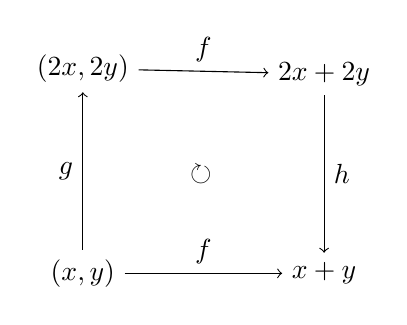
\begin{tikzpicture} \label{comm_diagram_ex}
\node (m) {$(x,y)$};
\node (fm) [right=2cm of m] {$x+y$};
\node (em) [above=2cm of m] {$(2x,2y)$};
\node (fem) [above=2cm of fm] {$2x+2y$};
\node(circarr) [above right=1cm of m]{$\circlearrowright$};
\draw[->] (m) to node {$f$} (fm);
\draw[->] (fem) to node {$h$} (fm);
\draw[->] (m) to node {$g$} (em);
\draw[->] (em) to node {$f$} (fem);
\end{tikzpicture}$
\end{center}

\end{itemize}

\

\section{Notes}
Cite Donald Knuth, Art of Computer Programming, Addison-Wesley Publishing Company, Reading, Massachusetts, second edition, pp 273-4 for representation of multivariate polynomials using linked lists.

\

Cite Gentry, Fellows and Koblitz, Dummit and Foote, Grobner Bases book, Henri Cohen, HPS, Lauter, Bayer/Stillman syzygies, Faugere FGb explanation, Barkee, PCRevisited, van Dijk/Gentry/Halevi/Vaikuntanathan(http://eprint.iacr.org/2009/616.pdf), Lang's \emph{Algebra}

\

Page 38 of HPS

\

Changed RAND to RAND2 after a bunch of tests already computed. Initially, we were using just products of random numbers to generate new random numbers, but there was an issue that if any of these random numbers were even, all subsequent ones would be as well, implying that most coefficients were probably even (since the bounds we use are powers of two). It is changed to increase by multiplying by a rand and also adding one. Also changed it to make constant coefficients non-zero, since constant coeffs help to hide the message. Also changed the coeffs of random polys to between coeffbd and 1 rather than coeffbd and coeffbd/2.

\

32749 is the largest prime usable in M2 for polynomial rings over finite fields

\

Note that coeffsize doesn't matter so much for Z/pZ, since arithmetic is all Z/pZ

\

Cite sage, M2, singular, c++, GMP, d3, Maple, Faugere's FGb package (http://www-polsys.lip6.fr/~jcf/Papers/ICMS.pdf), GMP manual

acknowledge Prof. Stillman for helpful conversation

\

Idea: get f.resultant(g,x) and f.resultant(g,y) to reduce encryptions by!~\cite{gentry-thesis} hi~\cite{becker}


\bibliography{biblio}{}
\bibliographystyle{plain}
\end{document}  